% !TeX program = tectonic-local
% !TeX encoding = UTF-8
% Nguồn: Chương 3.docx. Biên dịch bằng XeLaTeX hoặc LuaLaTeX.
% Giữ nguyên nội dung và biểu thức toán của bản nguồn.
% Sơ đồ Word được dựng lại bằng TikZ; ảnh nằm trong chuong3-assets/media/.
\documentclass[12pt,a4paper,oneside]{report}
\usepackage{fontspec}
\IfFontExistsTF{Times New Roman}{\setmainfont{Times New Roman}}{\setmainfont{TeX Gyre Termes}}
\usepackage[left=3cm,right=2cm,top=2.5cm,bottom=2.5cm]{geometry}
\usepackage{amsmath,amssymb}
\usepackage{graphicx}
\usepackage{setspace}
\usepackage{tikz}
\usetikzlibrary{arrows.meta,positioning,shapes.geometric}
\renewcommand{\chaptername}{Chương}
\renewcommand{\figurename}{Hình}
\renewcommand{\contentsname}{Mục lục}
\setcounter{secnumdepth}{2}
\setlength{\parindent}{1cm}
\setlength{\parskip}{4pt}
\setlength{\emergencystretch}{3em}
\onehalfspacing
\begin{document}
\setcounter{chapter}{2}

\chapter{Nhóm thuật toán dựa trên trường lực}

\section{Phương pháp trường thế nhân tạo (APF)}

- Phương pháp Artificial Potential Field (APF) mô phỏng không gian làm việc của robot như một trường năng lượng toán học, trong đó các vật cản đóng vai trò là các điểm có thế năng cao, còn mục tiêu là điểm có thế năng thấp nhất.

\begin{center}
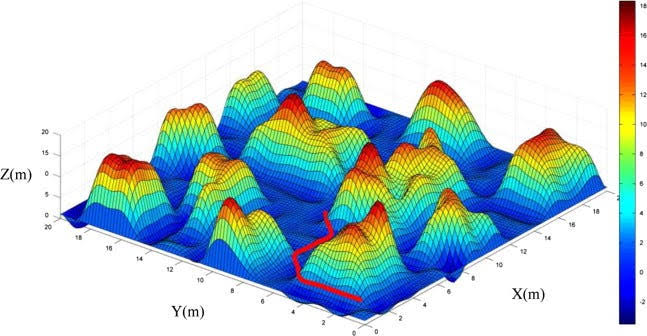
\includegraphics[width=0.85\linewidth,keepaspectratio]{chuong3-assets/media/image1.jpeg}
\end{center}

- Trong mô hình không gian của phương pháp APF, các vật cản có các đỉnh thế năng cao, đẩy robot ra xa, còn điểm đích là điểm có thế năng thấp nhất, kéo robot về phía nó. Nói cách khác, robot di chuyển theo hướng giảm thế năng cục bộ.

- Trong không gian này, ta quy ước \(q = \lbrack x,\ y\rbrack^{T}\) là vị trí hiện tại của robot,\({\ q}_{goal}\) là vị trí điểm đích, \({\ q}_{obs}\) là vị trí vật cản.

\subsection{Hàm thế hút \(\mathbf{\ U}_{\mathbf{att}}\)}

\begin{enumerate}
\def\labelenumi{\arabic{enumi}.}
\item
  Mô hình xác định thế năng của vật rắn tổng quát: \(U = \frac{1}{2}k{(\Delta x)}^{2}\) . Đối chiếu với mô hình không gian của thuật toán APF, ta có mô hình cơ bản của hàm thế nút:
\end{enumerate}

\[U_{att}(q) = \frac{1}{2}k_{att}.\left\| q - {\ q}_{goal} \right\|^{2}\]

*Trong đó: \(k_{att}\) là hệ số thế hút, tỉ lệ thuận với cường độ của lực hút

\(\left\| q - {\ q}_{goal} \right\|\) là khoảng cách Euclid giữa robot với điểm đích

- Lực hút lấy đạo hàm Gradient âm của thế năng \(F = - \nabla U\) , như vậy lực hút \(F_{att}\) do hàm thế hút sẽ là:

\[F_{att} = - \nabla U_{att}(q) = - k_{att}(q - {\ q}_{goal})\]

- Đặc điểm:

+ Lực hút tỉ lệ thuận với khoảng cách giữa robot và điểm đích. Khoảng cách càng lớn, lực kéo sẽ càng mạnh. Khi khoảng cách được thu hẹp, tức robot đến gần điểm đích, lực kéo giảm dần về 0 giúp robot dừng lại ở điểm đích một cách chính xác và mượt mà.

+ Khi robot ở quá xa so với điểm đích, tức khoảng cách lớn, \(F_{att}\) tăng lên rất lớn khiến robot bị mất ổn định về vận tốc. Đây là nhược điểm của mô hình hàm thế hút cơ bản.

\begin{enumerate}
\def\labelenumi{\arabic{enumi}.}
\setcounter{enumi}{1}
\item
  Để khắc phục điều này, ta có mô hình hàm thế nút dạng tuyến tính, sử dụng hàm dạng hình nón:
\end{enumerate}

\[U_{att}(q) = k_{att}.\left\| q - {\ q}_{goal} \right\|\]

Lấy là đạo hàm Gradient âm ta thu được lực hút:

\[F_{att}(q) = - k_{att}.\frac{q - {\ q}_{goal}}{\left\| q - {\ q}_{goal} \right\|}\]

- Đặc điểm:

+ Độ lớn lực \(\left| F_{att} \right| = k_{att}\) là một hằng số, nghĩa là robot sẽ di chuyển với một lực kéo cố định bất kể khoảng cách. Như vậy dù khoảng cách rất lớn thì robot vẫn ổn định.

+ Khi đến điểm đích, robot vẫn chịu tác dụng của \(F_{att}\) khiến robot không dừng lại, va đập hoặc rung lắc quanh \({\ q}_{goal}\). Đây là nhược điểm của mô hình tuyến tính.

\begin{enumerate}
\def\labelenumi{\arabic{enumi}.}
\setcounter{enumi}{2}
\item
  Mô hình hàm thế hút kết hợp:
\end{enumerate}

\[U_{att}(q) = \begin{cases}
\frac{1}{2}k_{att}.\left\| q - {\ q}_{goal} \right\|^{2} & \text{nếu } \left\| q - {\ q}_{goal} \right\|\  \leq d_{goal}\  \\
d_{goal}.k_{att}.\left\| q - {\ q}_{goal} \right\|\  - \frac{1}{2}k_{att}.{(d_{goal})}^{2} & \text{nếu } \left\| q - {\ q}_{goal} \right\|\  > d_{goal}\ 
\end{cases}\ \]

Với \(d_{goal}\) là ngưỡng khoảng cách giữa vị trí hiện tại của robot đến điểm đích do người lập trình tự thiết lập để chia không gian xung quanh điểm đích thành hai vùng điều khiển như trên.

- Lực hút tổng hợp:

\[F_{att}(q) = \begin{cases}
 - k_{att}.(q - {\ q}_{goal}) & \text{nếu } \left\| q - {\ q}_{goal} \right\|\  \leq d_{goal}\  \\
d_{goal}.k_{att}.\frac{q - {\ q}_{goal}}{\left\| q - {\ q}_{goal} \right\|} & \text{nếu } \left\| q - {\ q}_{goal} \right\|\  > d_{goal}\ 
\end{cases}\ \]

Với mô hình tổng hợp này, vừa có thể phát huy được điểm mạnh của hai mô hình trên cũng như là khắc phục được nhược điểm của những mô hình đó.

\subsection{Hàm thế đẩy \(\mathbf{\ U}_{\mathbf{rep}}\)}

- Trong mô hình không gian của thuật toán APF, bản chất của \({\ U}_{rep}\) là tạo ra thế năng xung quanh vật cản, có tác dụng tạo ra các vector lực tổng hợp đẩy robot đi ra xa.

- Mô hình hàm thế đẩy truyền thống được đưa ra bởi nhà khoa học robotic Oussama Khatib vào năm 1986. Mô hình \({\ U}_{rep}\) như sau (Khatib Model):

\[U_{rep}(q) = \begin{cases}
\frac{1}{2}k_{rep}.\left( \frac{1}{d(q)} - \frac{1}{\rho_{0}} \right)^{2} & \text{nếu } d(q) \leq \rho_{0} \\
0 & \text{nếu } d(q) > \rho_{0}
\end{cases}\ \]

*Trong đó:

\(k_{rep}\) : Hệ số thế đẩy. Tương tự như hệ số thế hút \(k_{att}\)

\(d(q)\): Khoảng cách ngắn nhất giữa robot và vật cản gần nhất \(\left( d(q) = \left\| q - {\ q}_{obs} \right\| \right)\)

\(\rho_{0}\) : Bán kính ảnh hưởng của vật cản. Nếu robot nằm ngoài phạm vi này sẽ không còn phát hiện vật cản, thế đẩy bằng 0. Điều này giúp robot không bị chịu thế đẩy của những vật cản ở quá xa không cần tránh.

Lực đẩy: Lấy Gradient âm của \({\ U}_{rep}\):

\[F_{rep}(q) = \begin{cases}
\frac{1}{2}k_{rep}.\left( \frac{1}{d(q)} - \frac{1}{\rho_{0}} \right).\frac{1}{d^{2}(q)}.\nabla d(q) & \text{nếu } d(q) \leq \rho_{0} \\
0 & \text{nếu } d(q) > \rho_{0}
\end{cases}\ \]

*Trong đó \(\nabla d(q) = \frac{q - {\ q}_{obs}}{\left\| q - {\ q}_{obs} \right\|}\) là vector đơn vị, hướng của lực đẩy \(F_{rep}\).

+ Khi khoảng cách \(d(q) \rightarrow 0\ \ \text{kéo theo}\ \ \frac{1}{d(q)} \rightarrow \infty\ \), lực đẩy tiến đến rất lớn giúp robot không va đụng vào vật cản.

+ Khi \(d(q) = \rho_{0}\): Lực đẩy giảm dần về 0, robot thực hiện chuyển sang vùng có thế hút mượt mà.

- Nhược điểm của mô hình truyền thống: Giả sử có vật cản ở gần điểm đích, điểm đích nằm trong bán kính \(\rho_{0}\) ảnh hưởng của vật cản. Theo lý thuyết lúc này\({\ F}_{att}\) giảm dần về 0 để robot dừng lại ở điểm đích, phải chịu thêm\({\ F}_{rep}\) khiến robot tiếp tục bị đẩy ra xa \(\Rightarrow\) Không thể tiếp cận điểm đích dù về mặt hình học là khả thi.

\subsection{Mô hình hàm thế tổng hợp \(\mathbf{\ U}_{\mathbf{total}}\) và lực đẩy tổng hợp \(\mathbf{\ F}_{\mathbf{total}}\)}

- Hàm thế tổng hợp là tổng của thế hút và tổng đại số thế đẩy của các vật cản. Mô hình thế năng tổng hợp:

\[U_{total}(q) = U_{att}(q) + \sum_{i = 1}^{N}{U_{rep,i}(q)}\]

*Trong đó N là số vật cản.

Lực đẩy tổng hợp là lấy đạo hàm gradient âm của hàm thế năng, ta có vector lực tổng hợp:

\[F_{total}(q) = - \nabla{\ U}_{total} = - {\nabla U}_{att}(q) - \sum_{i = 1}^{N}{{\nabla U}_{rep,i}(q)} = F_{att}(q) + \sum_{i = 1}^{N}{F_{rep,i}(q)}\]

Vector lực được tổng hợp theo quy tắc hình bình hành

\begin{center}
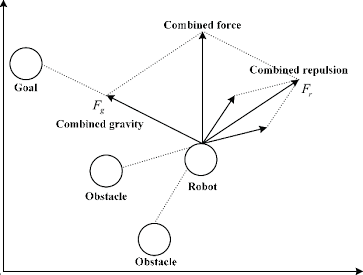
\includegraphics[width=0.85\linewidth,keepaspectratio]{chuong3-assets/media/image2.png}
\end{center}

- Robot sẽ cập nhật trạng thái chuyển động của sau mỗi chu kì \(\Delta t\) . Giả sử vị trí hiện tại của robot là \({\ q}_{k}\), vị trí tiếp theo sẽ là \({\ q}_{k + 1}\). Robot cập nhật vị trí theo phương pháp Hạ Gradient (Gradient Descent):

\[q_{k + 1} = q_{k} + \alpha.\frac{F_{total}(q_{k})}{\left\| F_{total}(q_{k}) \right\|}\]

*Trong đó \(\alpha\) là bước nhảy tối đa trong một chu kì (step size).

\section{Hiện tượng Local Minima, GNRON và sơ đồ khắc phục}

\subsection{Hiện tượng mục tiêu không thể tiếp cận điểm đích gần vật cản (GNRON)}

Quay trở lại với mô hình hàm thế đẩy Khatib, ta có lực đẩy \({\ F}_{rep}\) sinh ra bởi thế năng đẩy của vật cản:

\[F_{rep}(q) = \begin{cases}
\frac{1}{2}k_{rep}.\left( \frac{1}{d(q)} - \frac{1}{\rho_{0}} \right).\frac{1}{d^{2}(q)}.\nabla d(q) & \text{nếu } d(q) \leq \rho_{0} \\
0 & \text{nếu } d(q) > \rho_{0}
\end{cases}\ \]

- Lực đẩy phụ thuộc vào khoảng cách ngắn nhất giữa vị trí hiện tại của robot và điểm đích. Khi khoảng cách này nhỏ hơn bán kính ảnh hưởng của vật cản (\(\rho_{0}\)) thì robot sẽ chịu ảnh hưởng của lực đẩy.

- Trong trường hợp điểm đích \({\ q}_{goal}\) nằm trong bán kính ảnh hưởng của một hoặc nhiều vật cản xung quanh. Khi robot đến gần điểm đích,\({\ F}_{att}\) sẽ tiến dần về 0 để robot dừng lại dần, trong khi đó lực đẩy tổng hợp \({\ F}_{rep}\) sẽ lớn dần vì robot tiến vào trong bán kính ảnh hưởng

- Kết quả: Robot bị đẩy ra xa điểm đích, không thể tiếp cận điểm đích.

- Khắc phục: Để hạn chế ảnh hưởng của \({\ F}_{rep}\), thuật toán sẽ là nhân hàm thế đẩy \(U_{rep}\) với một hệ số \(\left\| q - q_{goal} \right\|^{2}\) phụ thuộc vào khoảng cách giữa robot hiện tại và điểm đích. Ta có mô hình hàm thế đẩy mới:

\[U_{rep}(q) = \begin{cases}
\frac{1}{2}k_{rep}.\left( \frac{1}{d(q)} - \frac{1}{\rho_{0}} \right)^{2}\ .\left\| q - q_{goal} \right\|^{2} & \text{nếu } d(q) \leq \rho_{0} \\
0 & \text{nếu } d(q) > \rho_{0}
\end{cases}\ \]

Lấy đạo hàm gradient âm của hàm thế năng ta thu được lực đẩy \({\ F}_{rep}\) mới gồm hai thành phần: \({\ F}_{rep1}(q)\) và \({\ F}_{rep2}(q)\), trong đó \({\ F}_{rep1}(q)\) chứa hệ số \(\left\| q - q_{goal} \right\|^{2}\) đóng vai trò lực đẩy,\({\ F}_{rep2}(q)\) đóng vai trò lực kéo robot về điểm đích.

Khi robot tiếp cận điểm đích, hệ số \(\left\| q - q_{goal} \right\|^{2}\) tiến dần về 0 kéo theo \({\ F}_{rep1}(q)\) cũng nhỏ dần, tạo điều kiện cho robot tiếp cận điểm đích mượt mà.

\subsection{Hiện tượng Cực tiểu cục bộ (Local Minima)}

- Trong đa số trường hợp, vector \({\overrightarrow{F}}_{att}\) kéo robot về phía điểm đích, trong khi \({\overrightarrow{F}}_{rep}\) đẩy robot tránh xa vật cản, giúp robot tự tránh vật cản và tiến về điểm đích.

- Tồn tại các điểm không gian đặc biệt mà tại đó lực kéo \({\overrightarrow{F}}_{att}\) có cùng độ lớn với tổng hợp của các vector \({\overrightarrow{F}}_{rep}\) nhưng có hướng ngược nhau \(\left( F_{att} + \sum_{}^{}{F_{rep} = 0} \right)\), \(F_{total} = 0\) - Kết quả: Robot đứng yên tại chỗ, rung lắc liên tục.

- Các trường hợp thường xảy ra:

+ Vật cản hình móng ngựa hoặc hình chữ U nằm giữa robot và điểm đích.

+ Nhiều vật cản xung quanh điểm đích tạo ra lực đẩy tổng hợp triệt tiêu với lực hút.

+ Hành lang hẹp hoặc rơi vào ngõ cụt.

+ Vật cản nằm thẳng dài dọc theo đường nối giữa robot và điểm đích.

*Phương pháp lực ảo điều hướng (Virtual Force)

- Phương pháp được thực hiện bằng cách sinh ra một vector lực xoáy vuông góc với lực đẩy \({\overrightarrow{F}}_{rep}\) của vật cản, có vai trò phá vỡ sự cân bằng của lực đẩy và lực kéo, tạo ra lực tổng hợp kéo robot di chuyển dọc theo đường bao của vật cản cho đến khi thoát khỏi vị trí đó.

- Các bước xử lý:

\begin{enumerate}
\def\labelenumi{\arabic{enumi}.}
\item
  \textbf{Kiểm tra trạng thái:}
\end{enumerate}

Trong mỗi chu kỳ, hệ thống sẽ liên tục kiểm tra các điều kiện để xác định xem robot có đang bị rơi vào Local Minima hay không:

• Vận tốc của robot \(v \approx 0\) , lực tổng hợp \(\left\| F_{total} \right\| < \varepsilon\ \)với \(\varepsilon\) có giá trị rất nhỏ.

• Khoảng cách từ robot đến điểm đích vẫn còn xa.

Trong khoảng thời gian \(\Delta t\), nếu cả hai điều kiện này liên tục thỏa mãn thì robot sẽ được xác định là đang rơi vào hiện tượng Local Minima.

\begin{enumerate}
\def\labelenumi{\arabic{enumi}.}
\setcounter{enumi}{1}
\item
  \textbf{Tính toán lực điều hướng ảo}: Lực điều hướng ảo \(F_{vir}\) có phương vuông góc với \({\overrightarrow{F}}_{rep}\), tạo ra vector lực tổng hợp kéo robot di chuyển dọc theo đường bao của vật cản
\end{enumerate}

Ma trận xoay \(R(\theta)\):

\[R(\theta) = \begin{bmatrix}
\cos\theta & - sin\theta \\
\sin\theta & \cos\theta
\end{bmatrix}\]

\({\overrightarrow{F}}_{vir}\bot{\overrightarrow{F}}_{rep}\) nên \(\theta = \pm \pi/2\) . Ma trận \(R(\theta)\) trở thành: \(R( \pm \pi/2) = \begin{bmatrix}
0 & - 1 \\
1 & 0
\end{bmatrix}\)

Nhân vector lực đẩy với ma trận trên ta có lực ảo:

\[F_{vir} = \  \pm \alpha.\begin{bmatrix}
0 & - 1 \\
1 & 0
\end{bmatrix}F_{rep} = \  \pm \alpha.\begin{bmatrix}
0 & {- F}_{rep\_ y} \\
F_{rep\_ x} & 0
\end{bmatrix}\]

\(\alpha\): Hệ số cường độ lực ảo

Ngoài ra để robot tự chọn đường di chuyển ngắn hơn khi trượt dọc theo đường bao vật cản, cần xác định tích có hướng của hai vector \(V = q_{goal} - q\) và \(Q = q_{obs} - q\)

\[Z = V_{x}.Q_{y} - V_{y}.Q_{x}\]

Nếu Z \textgreater{} 0, robot sẽ đi bên trái, ngược lại Z \textless{} 0 thì sẽ trượt sang phải.

\begin{enumerate}
\def\labelenumi{\arabic{enumi}.}
\setcounter{enumi}{2}
\item
  \textbf{Tổng hợp lực mới, cập nhật vị trí}
\end{enumerate}

- Hệ thống tạm thời dừng việc tính toán \(F_{total} = F_{att} + F_{rep}\), thay bằng \(F_{total} = F_{rep} + F_{vir}\) để đưa robot vượt qua vật cản

- Cập nhật vị trí: Sử dụng phương pháp Euler:

\[q_{k + 1} = q_{k} + v_{\max}.\frac{F_{total}}{\left\| F_{total} \right\|}.\Delta t\]

Trong đó:\(\ v_{\max}\) là vận tốc lớn nhất của robot

\(\Delta t\) : chu kỳ cập nhật vị trí

\begin{enumerate}
\def\labelenumi{\arabic{enumi}.}
\setcounter{enumi}{3}
\item
  \textbf{Liên tục kiểm tra điều kiện xem robot đã thoát khỏi trạng thái kẹt hay chưa}
\end{enumerate}

- Hệ thống liên tục kiểm tra, tính toán xem robot đã thoát khỏ Local Minima hay chưa, trả lại \(F_{total} = F_{att} + F_{rep}\), tránh việc robot đi một vòng rồi quay lại vị trí kẹt

- Điều kiện thoát: Vector lực hút \({\overrightarrow{F}}_{att}\) và vector lực đẩy \({\overrightarrow{F}}_{rep}\) tạo một góc nhỏ hơn 90°

Tích vô hướng:

\[\left( F_{att},\ F_{rep} \right) > 0\  \Leftrightarrow \ \ F_{att\_ x}.F_{rep\_ x} + F_{att\_ y}.F_{rep\_ y} > 0\]

Lược đồ thuật toán quay lại bước 1.

Lược đồ thuật toán giải quyết Local Minima:


\begin{center}
\begin{tikzpicture}[
  node distance=7mm,
  every node/.style={font=\small,align=center},
  process/.style={draw,rounded corners,text width=9cm,inner sep=5pt},
  decision/.style={draw,diamond,aspect=3,text width=5.3cm,inner sep=2pt},
  arrow/.style={-{Stealth},thick}
]
\node[decision] (check) {Kiểm tra trạng thái:\\robot bị kẹt?};
\node[process,below=of check] (virtual) {Đúng: Tính toán lực ảo\\[3pt]
$F_{vir}=\pm\alpha.\begin{bmatrix}0 & -F_{rep\_ y}\\F_{rep\_ x} & 0\end{bmatrix}$\\[3pt]
$Z=V_x.Q_y-V_y.Q_x$};
\node[process,below=of virtual] (update) {Tổng hợp lực mới, cập nhật vị trí\\[3pt]
$F_{total}=F_{rep}+F_{vir}$\\[3pt]
$q_{k+1}=q_k+v_{\max}.\dfrac{F_{total}}{\lVert F_{total}\rVert}.\Delta t$};
\node[decision,below=of update] (exit) {Kiểm tra điều kiện thoát kẹt\\[3pt]
$F_{att\_ x}.F_{rep\_ x}+F_{att\_ y}.F_{rep\_ y}>0$};
\node[process,below=of exit] (restore) {Đúng: Trả lại lực cũ\\[3pt]
$F_{total}=F_{att}+F_{rep}$};
\draw[arrow] (check) -- (virtual);
\draw[arrow] (virtual) -- (update);
\draw[arrow] (update) -- (exit);
\draw[arrow] (exit) -- (restore);
\draw[arrow] (check.east) -- ++(3.1,0) node[midway,above]{Sai} |- (check.north);
\draw[arrow] (exit.west) -- ++(-2.3,0) node[pos=0.3,above]{Sai} |- (virtual.west);
\draw[arrow] (restore.east) -- ++(1.4,0) |- (check.north);
\end{tikzpicture}
\end{center}

\end{document}
